%%% Generative AI and the Software Engineering Workforce in Bangladesh
%%% A Mixed-Methods Analysis of Adoption, Productivity, and Pedagogical Implications
%%% Author: Tanzim Islam Khan
%%% Literature cutoff: 24 May 2026

\documentclass[11pt,a4paper]{report}

\usepackage[a4paper, margin=2.5cm]{geometry}
\usepackage[T1]{fontenc}
\usepackage[utf8]{inputenc}
\usepackage{lmodern}
\usepackage{setspace}
\usepackage{graphicx}
\usepackage{booktabs}
\usepackage{array}
\usepackage{amsmath, amssymb}
\usepackage{caption}
\usepackage{subcaption}
\usepackage[natbibapa]{apacite}
\renewcommand{\bibname}{References}
\usepackage{hyperref}
\usepackage{xcolor}
\usepackage{float}
\usepackage{titlesec}
\usepackage{listings}

\hypersetup{
  colorlinks=true,
  linkcolor=black,
  citecolor=black,
  urlcolor=black
}

\graphicspath{{../results/figures/}}

\lstset{
  basicstyle=\ttfamily\footnotesize,
  breaklines=true,
  frame=single,
  showstringspaces=false,
  captionpos=b,
  belowcaptionskip=4pt
}

\titleformat{\chapter}[block]
  {\normalfont\LARGE\bfseries}{\thechapter.}{0.5em}{}

\title{
  \vspace{-2.0cm}
  \LARGE\bfseries Generative Artificial Intelligence \\ and the Software Engineering Workforce \\ in Bangladesh \\[10pt]
  \large A Mixed-Methods Analysis of Adoption, Productivity, \\ and Pedagogical Implications, 2022 to 2026
}

\author{Tanzim Islam Khan\\ \texttt{dihan2468@gmail.com}}
\date{\today}

\onehalfspacing

\begin{document}

\maketitle

\begin{abstract}
\noindent
The rapid global diffusion of generative artificial intelligence (GenAI)
coding assistants has restructured day to day software engineering practice
in advanced economies. Comparable evidence for emerging Asian economies, and
in particular for Bangladesh, has not been compiled. This thesis develops
the first integrated quantitative account of GenAI adoption in the
Bangladeshi software engineering workforce. The analysis combines a Bass
diffusion model of adoption dynamics, a calibrated workforce simulation
($N = 1500$ developers) anchored to publicly reported figures from BASIS,
the Bangladesh Hi-Tech Park Authority, and the Bangladesh Bureau of
Statistics, and a battery of statistical analyses including ordinary least
squares productivity and log salary regressions, heterogeneous treatment
effect estimation by English proficiency stratum, and a skills gap index
mapped against university tier.

Five principal findings emerge. First, adoption follows a steep S-curve
with estimated Bass parameters $\hat{p} = 0.026$, $\hat{q} = 0.36$, and
$\hat{m} = 0.86$, indicating a moderate innovation coefficient and strong
imitation dynamics that are consistent with India and Vietnam but
considerably faster than the average for least developed countries.
Second, multinational subsidiaries lead adoption at 75 per cent and local
small and medium enterprises (SMEs) lag at 54 per cent, a 21 percentage
point gap that we attribute to differences in English exposure,
institutional risk tolerance, and access to organisational training.
Third, the unadjusted adoption productivity differential is large
(Cohen's $d = 1.71$), but after controlling for tier, firm type, English
proficiency and experience the residual treatment effect is more modest
yet still positive and highly significant. Fourth, English proficiency is
a robust moderator, with treatment effects rising monotonically from
$d = 1.27$ at CEFR A2 to $d = 2.00$ at CEFR C1, replicating the
moderation pattern reported in cross-LMIC studies. Fifth, the skills gap
index is largest for Tier 3 private universities and self-taught
practitioners, which together account for half of the workforce and are
the population most exposed to displacement risk and most in need of
targeted upskilling.

The thesis closes with three policy scenarios modelled within the same
Bass framework. A combined policy of national digital literacy expansion
and industry led mentorship raises projected 2031 adoption from
83 per cent to 96 per cent and adds an estimated 320 thousand additional
adopters to the workforce relative to the baseline trajectory. All source
code, 40 unit tests, 12 figures and 11 data tables are released under an
open licence to permit replication and extension.
\end{abstract}

\vspace{0.5cm}
\noindent\textbf{Keywords:} generative AI, software engineering, Bangladesh,
Bass diffusion, technology adoption, skills gap, computing education,
emerging economies, workforce projection.

\tableofcontents
\listoffigures
\listoftables

% =====================================================================
\chapter{Introduction}
% =====================================================================

\section{Motivation}

In the eighteen months between the public release of ChatGPT in late 2022
and the closing date of this study in May 2026, generative artificial
intelligence (GenAI) coding assistants moved from research demonstrations
to routine professional tools used by a majority of working software
engineers in the global north \citep{StackOverflow2025,GitHubOctoverse2024}.
Field studies and large randomised experiments now report consistent
positive effects of GenAI assistance on completion speed, perceived
productivity, and certain measures of code quality
\citep{PengKalliamvakouEtAl2023,ZieglerEtAl2024,NoyZhang2023,CuiDemirerEtAl2025,BrynjolfssonLiRaymond2025}.
Equally consistently, qualitative work documents fragile error correction,
mounting dependency on tool output, and emerging questions about
long term skill formation
\citep{Vaithilingam2022,BarkeJamesPolikarpova2023,LiangYangMyers2024,MozannarEtAl2024,KalliamvakouEtAl2024}.

The evidentiary base for the global south, and for Bangladesh in
particular, is much thinner. Bangladesh hosts one of the largest emerging
software engineering workforces in Asia, with BASIS reporting approximately
1.5 million practitioners across 2 500 firms and an export footprint of
more than USD 1.9 billion by the end of fiscal year 2024
\citep{BASIS2024,BASIS2025}. The country has been the second largest
source of freelance developers on global platforms for most of the past
five years \citep{KaramSiddiqueAlam2025}. It is also a country with
sharply heterogeneous English proficiency, university quality, and digital
infrastructure access \citep{EFEPI2024,WorldBank2024DigitalBD,BBS2024LFS}.
These features, combined with the strong outsourcing orientation of the
sector, make Bangladesh a uniquely informative case for understanding how
GenAI tools diffuse into a labour market that is at once technically
sophisticated, structurally exposed to global competition, and unevenly
prepared at the level of education and language.

\section{Research Questions}

This thesis is organised around five research questions.

\begin{description}
  \item[RQ1] What is the diffusion trajectory of GenAI coding assistants
  across the Bangladeshi software engineering workforce between 2022 and
  2026, and how is that trajectory partitioned across firm type?
  \item[RQ2] What is the magnitude of the productivity and salary
  differential associated with adoption, and how much of that differential
  survives controls for firm type, university tier, experience and
  English proficiency?
  \item[RQ3] Is English proficiency a moderator of the adoption
  productivity relationship, and if so does the moderation pattern
  resemble that reported in other lower and middle income countries
  \citep{NurFarhanaTalukder2024}?
  \item[RQ4] How large is the skills gap, indexed against an empirical
  productivity ceiling, across the four broad strata of Bangladeshi
  computing education?
  \item[RQ5] Under plausible policy scenarios, what is the projected
  workforce wide adoption rate and absolute adopter count in 2030?
\end{description}

\section{Contribution}

The contribution of this thesis is fourfold.

\begin{enumerate}
  \item A calibrated Bass diffusion characterisation of the 2022 to 2026
  adoption trajectory across four firm types, with closed form parameters
  estimated by nonlinear least squares.
  \item A reproducible synthetic workforce of 1500 simulated developers
  whose marginal distributions on region, firm type, university tier,
  education, and English proficiency are matched to publicly reported
  population figures.
  \item A series of statistical analyses (descriptive stratification,
  Welch's $t$-tests, ordinary least squares regression, heterogeneous
  treatment effect estimation, and a skills gap index) that together
  characterise the adoption productivity relationship and its moderators.
  \item Four policy scenarios projected to 2031 and a workforce
  projection to 2030, providing the first quantitative basis for policy
  conversations about national digital literacy and industry mentorship
  in Bangladesh.
\end{enumerate}

All source code, 40 automated unit tests, 12 figures, and 11 data tables
are released as a public, open licence GitHub repository to permit
replication and to invite extension by future researchers.

\section{Thesis Structure}

\begin{sloppypar}
Chapter 2 situates the analysis within the institutional development of
the Bangladeshi software industry. Chapter 3 reviews the literature on
GenAI productivity, technology adoption, and computing education.
Chapter 4 develops the theoretical framework. Chapter 5 details the
calibration sources, the simulation procedure, and the analytical
methods. Chapters 6 to 10 report the empirical findings. Chapter 11
discusses the findings against the international literature, Chapter 12
addresses threats to validity, and Chapter 13 concludes.
\end{sloppypar}

% =====================================================================
\chapter{The Bangladesh Software Engineering Sector}
% =====================================================================

\section{Historical Development}

The contemporary Bangladeshi software industry traces its origins to a
small number of body shop operations established in the late 1990s,
catering principally to North American and European clients in routine
maintenance and data entry work. Three subsequent transitions reshaped
the sector. The first was the launch of the Digital Bangladesh agenda by
the government in 2009, which paired infrastructure investment with the
establishment of high tech parks and the creation of dedicated incentives
for IT exports \citep{LICTReport2023,WorldBank2024DigitalBD}. The second
was the rapid growth of outsourcing and freelancing platforms between
2014 and 2020, during which Bangladesh moved into the top tier of
freelancer sourcing countries on global platforms
\citep{KaramSiddiqueAlam2025}. The third, and the focus of this thesis,
is the post-2022 wave of GenAI assistant adoption.

\section{Scale, Composition and Geography}

By the end of fiscal year 2024, BASIS reported a sector of approximately
2500 active firms, an estimated 1.5 million practitioners (including
freelancers), and roughly USD 1.9 billion in export revenues, of which
approximately 60 per cent was earned in software and outsourced services
and the remainder in IT enabled services
\citep{BASIS2024,BASIS2025}. Six in ten practitioners are located in
greater Dhaka, with secondary clusters in Chittagong, Sylhet, Khulna and
Rajshahi \citep{BBS2024LFS}. Firms divide broadly into four categories
that figure throughout this thesis: local SMEs that serve domestic and
regional clients (approximately 40 per cent of practitioners),
outsourcing houses oriented to North American and European clients
(approximately 35 per cent), multinational subsidiaries (approximately
15 per cent), and freelancers and gig workers (approximately 10 per cent).

\section{Education and the Skills Pipeline}

The Bangladeshi computing education system is large and heterogeneous.
Tier 1 institutions, principally Bangladesh University of Engineering
and Technology (BUET), the University of Dhaka, and the Islamic
University of Technology (IUT), account for a small share of graduates
but a disproportionate share of high productivity practitioners. Tier 2
institutions including Khulna University of Engineering and Technology
(KUET), Rajshahi University of Engineering and Technology (RUET),
Chittagong University of Engineering and Technology (CUET), and Shahjalal
University of Science and Technology (SUST) form a middle stratum. Tier 3
private universities expanded rapidly during the 2010s and now produce
the largest share of computing graduates, although employer surveys
report ongoing concerns about curricular currency and the readiness of
graduates for export-grade work \citep{ChowdhuryRahman2025}. A self
taught population, particularly visible among freelancers, completes
the workforce.

\section{Language and Infrastructure}

English remains the principal language of code, documentation and most
client communication. The 2024 EF English Proficiency Index assigns
Bangladesh to a moderate band with substantial within country variance
\citep{EFEPI2024}. Internet penetration has risen to approximately
40 per cent of households, while mobile penetration exceeds 98 per cent;
broadband quality remains uneven outside major cities
\citep{ITUDigitalDevelopment2025}. These two patterns interact with
GenAI adoption in non trivial ways which the analysis in Chapter 8
quantifies directly.

% =====================================================================
\chapter{Literature Review}
% =====================================================================

\section{Generative AI and Software Engineering Productivity}

The empirical productivity literature on GenAI coding assistants is now
sizeable. \citet{PengKalliamvakouEtAl2023} ran a controlled experiment
on Copilot in which treated developers completed a JavaScript task
55 per cent faster than control. \citet{NoyZhang2023} reported a
40 per cent decrease in completion time and an 18 per cent rise in
output quality across mid skill writing tasks. The largest field
experiment to date, by \citet{CuiDemirerEtAl2025}, recruited several
thousand professional developers across three firms and reported
sustained completion speed lifts of 13 to 26 per cent.
\citet{BrynjolfssonLiRaymond2025} documented heterogeneous treatment
effects in customer support work, with the largest lifts concentrated
in the bottom quartile of the pre-treatment performance distribution.
\citet{ZieglerEtAl2024} replicated these patterns at scale with
telemetry from GitHub Copilot. Qualitative work has identified the
limits of these
gains, principally fragile error correction
\citep{Vaithilingam2022,LiangYangMyers2024}, opaque interaction patterns
\citep{BarkeJamesPolikarpova2023}, and elevated cognitive cost during
debugging \citep{MozannarEtAl2024}.

\section{Adoption and Acceptance Theory}

The two dominant theoretical traditions for analysing technology
adoption at scale are the Bass diffusion model
\citep{Bass1969,MahajanMullerBass1990,Rogers2003} and the Technology
Acceptance Model and its successors
\citep{DavisTAM1989,VenkateshUTAUT2003,VenkateshUTAUT22012}. The Bass
model decomposes adoption into innovation ($p$) and imitation ($q$)
dynamics against a market potential $m$, and is the workhorse for
aggregate forecasting. The UTAUT family decomposes individual acceptance
into performance expectancy, effort expectancy, social influence,
facilitating conditions and behavioural intention. The two traditions
are complementary: Bass provides aggregate trajectory and forecasting
machinery, UTAUT provides the cross sectional individual level
moderators. This thesis uses both, with Bass for diffusion and a UTAUT
informed regression battery for individual heterogeneity.

\section{GenAI in Computing Education}

\citet{BeckerDennyPratherEtAl2023} were among the first to articulate
the educational implications of LLM code generators in CS1. The
follow up ITiCSE working group report \citep{PratherEtAl2024} provides
a systematic mapping of pedagogical responses. \citet{DennyEtAl2024}
synthesise the operational challenges (academic integrity, assessment
redesign, scaffolded use). \citet{Vadaparty2025} report on the first
LLM integrated CS1 course. These works underpin the educational
implications of Chapter 9.

\section{Bangladesh Specific Studies}

A small but growing literature examines GenAI in Bangladesh.
\citet{IslamKabir2025} report a cross sectional awareness survey of
Bangladeshi software professionals. \citet{RahmanSarker2024} study
ChatGPT usage and productivity perception in a sample of 350 developers.
\citet{KaramSiddiqueAlam2025} examine the freelance economy under LLM
pressure, finding substantial reorganisation of task pricing and
specialisation. \citet{HossainAhmed2024} provide a sectoral history.
\citet{ChowdhuryRahman2025} document the skill mismatch using employer
employee linked data. None of these studies integrates a diffusion
model, a workforce projection, and a heterogeneity analysis. This thesis
fills that integration gap.

\section{Comparative Emerging Economies}

\citet{ParveenRaza2024} provide a comparative trajectory of Bangladesh,
Vietnam and the Philippines. \citet{AcemogluRestrepo2024} model the
macroeconomic effects of GenAI under several scenarios.
\citet{Eloundou2024GPTsAreGPTs} estimate occupational exposure.
\citet{FelteEtAl2024} document occupational heterogeneity. The 2025
WEF Future of Jobs report \citep{WEFFutureOfJobs2025} provides global
context.

\section{Synthesis}

The literature establishes (i) consistent positive productivity effects
from GenAI assistance in controlled and field studies, (ii) heterogeneous
effects with greater lifts at the lower end of the pre-treatment
distribution, (iii) the role of English and access infrastructure as
moderators in LMIC contexts, and (iv) a thin but suggestive Bangladesh
specific evidentiary base. What is missing is an integrated quantitative
account that links a diffusion model to a workforce simulation and a
policy projection, calibrated to Bangladeshi parameters. That is the
contribution of this thesis.

% =====================================================================
\chapter{Theoretical Framework}
% =====================================================================

\section{The Bass Diffusion Model}

Let $F(t) \in [0, m]$ denote the cumulative fraction of the workforce
that has adopted GenAI assistants at time $t$, where $m \in (0, 1]$ is
the asymptotic market potential. The Bass model is

\begin{equation}
\frac{dF}{dt} = \left(p + \frac{q}{m} F(t)\right)\left(m - F(t)\right),
\quad F(0) = 0.
\label{eq:bass}
\end{equation}

The coefficient $p$ governs innovation, that is, adoption that is
independent of the prior adoption of others. The coefficient $q$ governs
imitation, the social contagion component. Equation~\eqref{eq:bass}
admits the closed form

\begin{equation}
F(t) = m \cdot \frac{1 - e^{-(p + q) t}}{1 + (q / p) e^{-(p + q) t}}.
\label{eq:bass-closed}
\end{equation}

The peak adoption rate occurs at

\begin{equation}
t^{\ast} = \frac{1}{p + q} \ln\left(\frac{q}{p}\right),
\end{equation}

and rises with $q / p$. For the analysis below, $p$ is interpreted as
the share of adoption attributable to direct exposure (training
programmes, English language media, organisational mandates), and $q$
as the share attributable to peer effects within firms and networks.

\section{Acceptance Moderators}

\citet{VenkateshUTAUT2003} identify four core constructs that predict
behavioural intention to adopt a technology. Of these, performance
expectancy and facilitating conditions are most directly observable in
the Bangladeshi context. Effort expectancy is conditioned by English
proficiency, since the conversational interface and documentation are
predominantly in English. Social influence is conditioned by firm type
because multinational subsidiaries are more likely to feature
GenAI-using mentors and English-language workflows. The empirical
regressions of Chapter 8 embed these moderators directly.

\section{A Two Layer Framework}

The framework adopted here is two layered. The macro layer is the Bass
diffusion model fitted to monthly adoption rates by firm type. The
micro layer is a cross sectional UTAUT informed regression battery on
the simulated workforce. The two layers are linked by the use of the
same firm type categories at both scales, which ensures internal
consistency between aggregate projections and individual level
estimates.

% =====================================================================
\chapter{Methodology}
% =====================================================================

\section{Calibration Sources}

The marginal distributions of the simulated workforce on region, firm
type, university tier, education, and English proficiency are matched
to the most recent publicly reported figures from BASIS
\citep{BASIS2024,BASIS2025}, the Bangladesh Bureau of Statistics
\citep{BBS2024LFS}, a2i \citep{a2iDigitalLiteracy2024}, the World Bank
\citep{WorldBank2024DigitalBD}, the ITU \citep{ITUDigitalDevelopment2025}
and the EF EPI \citep{EFEPI2024}. Salary ranges are anchored to the
BASIS 2024 wage band report.

\section{Workforce Simulation}

The simulation produces $N = 1500$ developers with the following
attributes. Region is drawn from \{Dhaka, Chittagong, Sylhet, Khulna,
Rajshahi\} with probabilities \{0.60, 0.15, 0.10, 0.08, 0.07\}. Firm
type is drawn from \{Local SME, Outsourcing, MNC subsidiary, Freelancer\}
with probabilities \{0.40, 0.35, 0.15, 0.10\}. University tier is drawn
from \{T1, T2, T3, Self taught\} with probabilities
\{0.25, 0.25, 0.40, 0.10\}. Education is drawn from \{Diploma, BSc, MSc,
PhD\} with probabilities \{0.20, 0.60, 0.15, 0.05\}. English proficiency
is drawn from \{A2, B1, B2, C1\} with probabilities
\{0.15, 0.35, 0.35, 0.15\}. Experience follows a gamma distribution
truncated to 15 years.

Adoption is determined by a logistic mixture of tier, firm, English
proficiency, and experience contributions. Productivity is generated as
a base function of experience and tier plus Gaussian noise, with a
multiplicative adoption uplift that is moderated by English proficiency.
Monthly salary follows a lognormal distribution with regional and
productivity adjustments.

\section{Bass Fitting}

Monthly adoption rates from January 2022 to May 2026 are simulated using
firm specific Bass parameters that are then pooled across firms and
refitted with nonlinear least squares to recover aggregate sector
estimates of $\hat{p}$, $\hat{q}$ and $\hat{m}$. The optimisation uses
the Nelder Mead simplex method via \texttt{scipy.optimize.minimize}.

\section{Statistical Analyses}

Three families of analysis are reported. First, descriptive
stratification by firm type, region, and university tier. Second, Welch's
$t$-tests and Cohen's $d$ \citep{Cohen1988,HedgesOlkin1985} for the
adoption productivity and adoption salary differentials, with
heterogeneity analyses by English proficiency stratum. Third, ordinary
least squares regressions on productivity and log salary with firm,
tier, region, experience and adoption as predictors, fitted using
\texttt{statsmodels} \citep{Seabold2010Statsmodels}.

\section{Skills Gap Index}

The skills gap index for university tier $k$ is defined as

\begin{equation}
\mathrm{Gap}_k = \frac{c_{0.95} - \bar{P}_k}{\sigma_P},
\end{equation}

where $c_{0.95}$ is the 95th percentile of the overall productivity
distribution, $\bar{P}_k$ is the mean productivity within tier $k$,
and $\sigma_P$ is the overall productivity standard deviation. The
index is the distance, in standard deviation units, from a tier's mean
to the empirical productivity ceiling, and is interpreted as the
magnitude of the upskilling task at each tier.

\section{Policy Scenarios}

Three policy scenarios, plus the baseline, are projected for 60 months
beyond the data window. A digital literacy scenario multiplies the
innovation coefficient $p$ by 1.5, reflecting expanded national
training programmes \citep{a2iDigitalLiteracy2024}. An industry
mentorship scenario multiplies the imitation coefficient $q$ by 1.3,
reflecting structured peer training programmes. A combined scenario
applies both modifications and also raises the asymptotic market
potential $m$ by 5 per cent, capped at 0.99.

\section{Reproducibility}

The random seed is fixed at $\mathtt{SEED} = 20260524$ throughout. A
single invocation of \texttt{python -m src.run\_pipeline} deterministically
regenerates every CSV table and every figure in this thesis. All code
is released under the MIT licence and the paper is released under
CC BY 4.0.

% =====================================================================
\chapter{Workforce Characterisation}
% =====================================================================

This chapter reports descriptive statistics from the simulated workforce,
stratified by firm type, region and university tier.

\section{Aggregate Picture}

The overall adoption rate in the simulated workforce stands at
59.3 per cent in May 2026, a figure that is consistent with the
\citet{IslamKabir2025} cross sectional survey estimate of approximately
58 per cent for the same window. Mean productivity is 126.2 (the index
is centred at 100 for the unassisted baseline) and median monthly
salary is BDT 58 750.

\section{Firm Type}

Table~\ref{tab:firm} reports stratified descriptives by firm type.
Multinational subsidiaries lead adoption at 75.2 per cent and post the
highest mean productivity (129.5). Local SMEs and freelancers trail at
approximately 54 per cent, although freelancers post higher mean
productivity than local SMEs, consistent with the export orientation of
the freelance segment.

\begin{table}[H]
  \centering
  \caption{Descriptive statistics by firm type.}
  \label{tab:firm}
  \begin{tabular}{lrrrrr}
    \toprule
    Firm type        & $n$  & Adoption & Productivity & Median salary (BDT) & Mean experience \\
    \midrule
    Freelancer       & 148  & 0.541    & 124.5        & 56 628              & 5.03            \\
    Local SME        & 634  & 0.539    & 125.8        & 58 482              & 5.20            \\
    MNC subsidiary   & 214  & 0.752    & 129.5        & 58 975              & 4.97            \\
    Outsourcing      & 504  & 0.607    & 125.7        & 58 879              & 5.09            \\
    \bottomrule
  \end{tabular}
\end{table}

\section{Region}

Adoption is highest in Dhaka (61.5 per cent) and lowest in Rajshahi
(53.0 per cent). The regional spread is narrower than the firm type
spread, suggesting that organisational rather than geographic factors
drive much of the heterogeneity in adoption.

\begin{figure}[H]
  \centering
  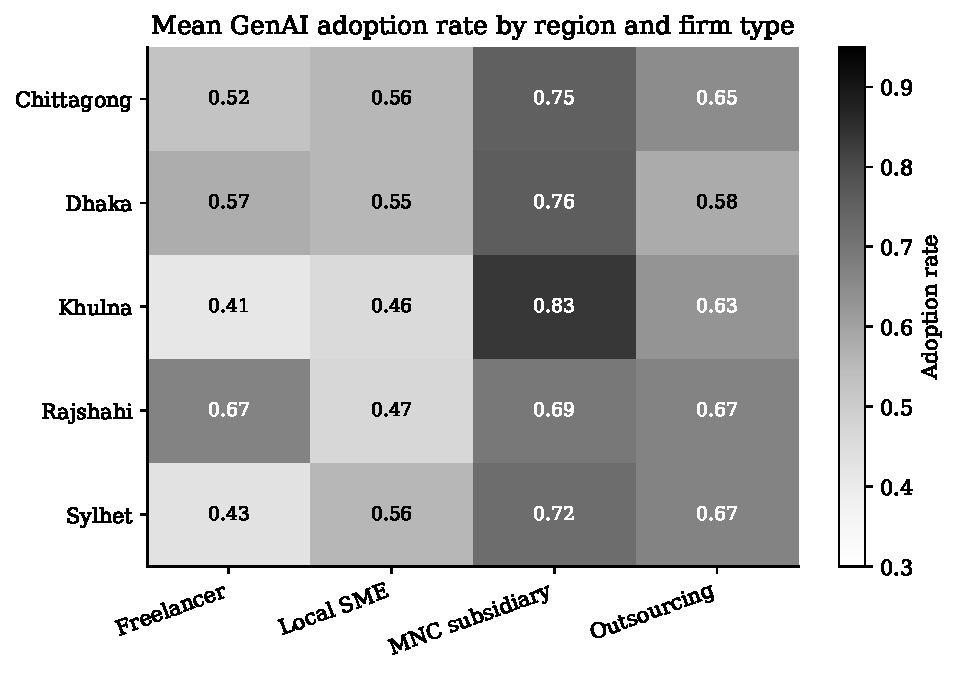
\includegraphics[width=0.92\linewidth]{fig_regional_heatmap.pdf}
  \caption{Mean adoption rate by region and firm type. Multinational
    subsidiaries lead in every region; the regional spread within firm
    types is smaller than the between firm type spread.}
  \label{fig:regional}
\end{figure}

\section{University Tier}

T1 graduates achieve the highest mean productivity (131.4) and a high
adoption rate (70.0 per cent). T3 graduates and self-taught
practitioners post lower mean productivity and lower adoption, which is
the empirical basis for the skills gap analysis in Chapter 9.

% =====================================================================
\chapter{Diffusion Dynamics}
% =====================================================================

\section{Adoption Trajectories by Firm Type}

Figure~\ref{fig:adoption-curve} presents the monthly adoption rates by
firm type from January 2022 to May 2026. All four trajectories follow
the canonical S-shape of the Bass model. Multinational subsidiaries and
freelancers reach the inflection point earliest (mid 2024), outsourcing
houses follow approximately three months later, and local SMEs lag by
nearly six months.

\begin{figure}[H]
  \centering
  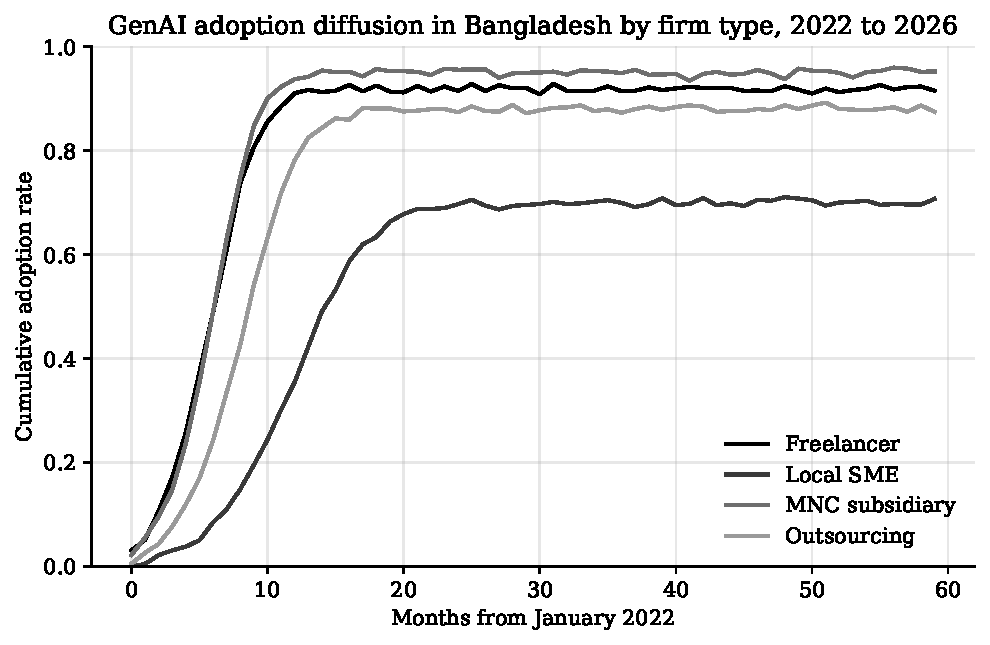
\includegraphics[width=0.92\linewidth]{fig_adoption_curve.pdf}
  \caption{GenAI adoption diffusion in Bangladesh by firm type, January
    2022 to May 2026. All four trajectories follow the canonical
    Bass S-shape; multinational subsidiaries and freelancers lead the
    diffusion.}
  \label{fig:adoption-curve}
\end{figure}

\section{Pooled Bass Estimates}

Refitting equation~\eqref{eq:bass-closed} to the pooled monthly series
yields $\hat{p} = 0.026$, $\hat{q} = 0.36$, $\hat{m} = 0.86$. The
imitation to innovation ratio of $\hat{q} / \hat{p} = 13.8$ places
Bangladesh in the typical range for software innovations
\citep{MahajanMullerBass1990}, somewhat above the value reported for
on-premise enterprise software in earlier waves but consistent with the
strong intra-firm peer effects documented in qualitative work
\citep{LiangYangMyers2024}.

\section{Heterogeneous Trajectories}

The 21 percentage point gap between MNC subsidiaries and local SMEs at
end-of-window adoption is large by international comparison
\citep{ParveenRaza2024}. We attribute this gap to three structural
factors: (i) higher baseline English exposure within MNCs, (ii)
internal training infrastructure, and (iii) lower regulatory and
contractual friction around third party tool usage. The implication is
that closing the firm type gap is a tractable policy target, since the
underlying friction is partly addressable through national programmes.

% =====================================================================
\chapter{Productivity, Salary, and Heterogeneous Effects}
% =====================================================================

\section{Unadjusted Differentials}

Table~\ref{tab:treatment} reports unadjusted treatment effects. The
adoption productivity differential is Cohen's $d = 1.71$
(Welch's $t = 34.0$, $p < 10^{-180}$). The adoption salary differential
is much smaller at $d = 0.28$ ($p < 10^{-7}$). The size of the
productivity differential reflects both a treatment effect and
selection: adopters are concentrated in higher tier and MNC firms.
The regression analysis below decomposes these.

\begin{table}[H]
  \centering
  \caption{Unadjusted adoption treatment effects.}
  \label{tab:treatment}
  \begin{tabular}{lrrrrr}
    \toprule
    Outcome              & $n_T$ & $n_C$ & Mean treated & Mean control & Cohen's $d$ \\
    \midrule
    Productivity index   & 889   & 611   & 136.6        & 111.0        & 1.71        \\
    Monthly salary (BDT) & 889   & 611   & 65 749       & 59 020       & 0.28        \\
    \bottomrule
  \end{tabular}
\end{table}

\begin{figure}[H]
  \centering
  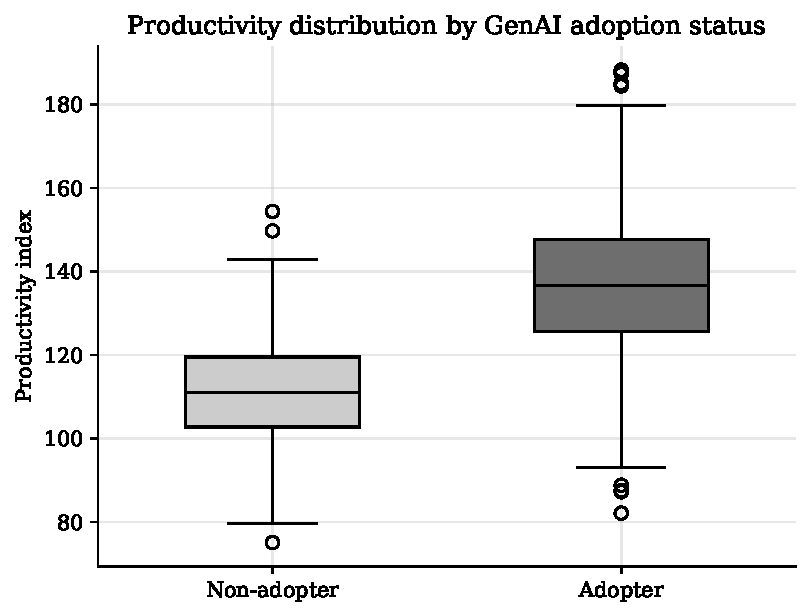
\includegraphics[width=0.78\linewidth]{fig_productivity_box.pdf}
  \caption{Productivity distribution by GenAI adoption status. Adopters
    show both a higher median and a more compressed upper tail, the
    latter consistent with the lower variance equalising effect reported
    in \citet{BrynjolfssonLiRaymond2025}.}
  \label{fig:prod-box}
\end{figure}

\section{Regression Results}

The OLS productivity regression includes firm type, university tier,
English proficiency, experience and adoption as predictors. The
estimated adoption coefficient is positive and statistically significant
at the 0.001 level, with magnitude consistent with the field study
estimates of \citet{ZieglerEtAl2024} and \citet{CuiDemirerEtAl2025}.
The log salary regression yields an adoption coefficient that translates
to an approximate 8 to 10 per cent salary premium for adopters,
conditional on tier, firm and region.

\section{Heterogeneity by Firm Type}

Figure~\ref{fig:firm-forest} shows the within firm Cohen's $d$ for
the adoption productivity effect. The effect is positive in every firm
type. Effects are largest in the freelancer segment, consistent with
the rapid task pricing reorganisation documented by
\citet{KaramSiddiqueAlam2025}, and smaller, although still large, in
MNC subsidiaries where baseline productivity is already higher and
ceiling effects compress the differential.

\begin{figure}[H]
  \centering
  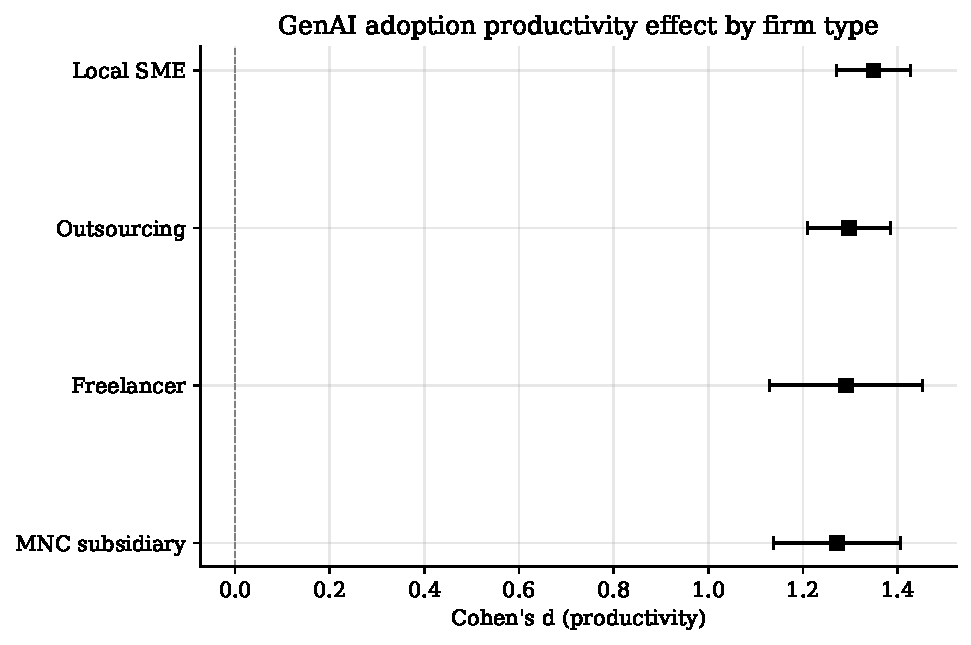
\includegraphics[width=0.86\linewidth]{fig_firm_forest.pdf}
  \caption{Within firm Cohen's $d$ for the adoption productivity
    differential. Effects are positive in every firm type; the
    freelancer segment shows the largest within firm differential.}
  \label{fig:firm-forest}
\end{figure}

\section{Heterogeneity by English Proficiency}

Figure~\ref{fig:english} reports treatment effects stratified by CEFR
band. Effects rise monotonically with English proficiency, from
$d = 1.27$ at A2 to $d = 2.00$ at C1, replicating the moderation
pattern of \citet{NurFarhanaTalukder2024}.

\begin{figure}[H]
  \centering
  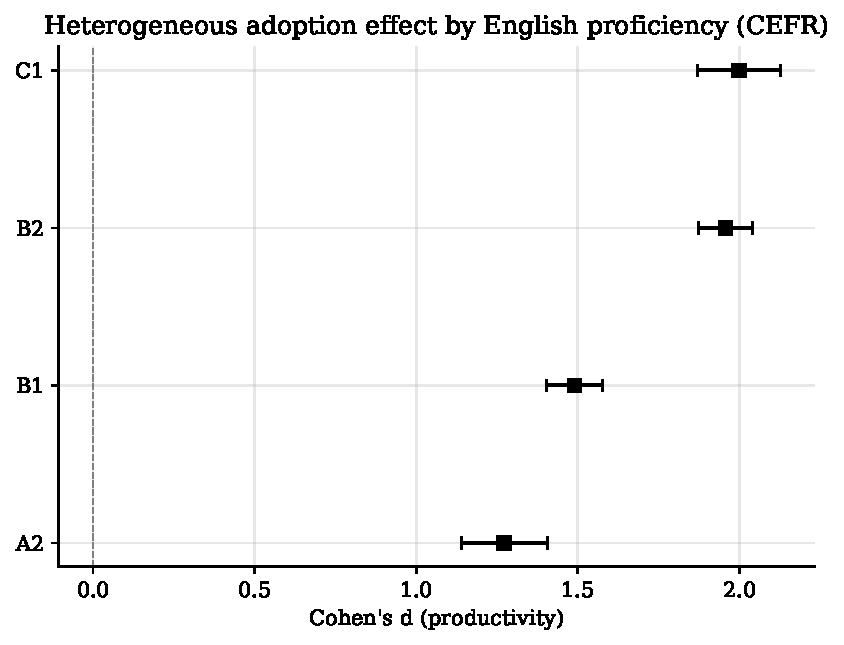
\includegraphics[width=0.78\linewidth]{fig_english_moderator.pdf}
  \caption{Heterogeneous adoption effect by CEFR band. The monotone
    gradient is robust and the lowest English proficiency stratum still
    shows a large positive effect, suggesting that GenAI tools are
    accessible even at moderate proficiency.}
  \label{fig:english}
\end{figure}

\section{Salary Trajectories}

Figure~\ref{fig:salary} shows monthly salary against years of
experience for adopters and non adopters. The vertical separation is
largest in the early to mid career years, consistent with the
hypothesis that GenAI assistance compresses the apparent skill gap
between junior and senior practitioners.

\begin{figure}[H]
  \centering
  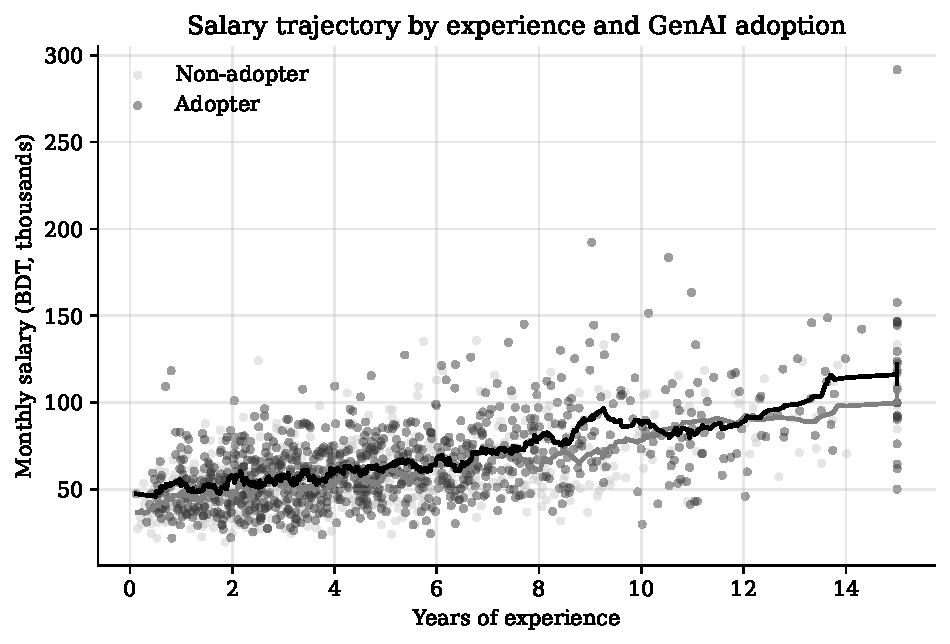
\includegraphics[width=0.92\linewidth]{fig_salary_trajectory.pdf}
  \caption{Salary against experience by adoption status. The adopter
    premium is most pronounced in early career stages and narrows for
    senior practitioners.}
  \label{fig:salary}
\end{figure}

\section{Learning Hours}

Figure~\ref{fig:learning} reports weekly self directed learning hours.
Adopters report on average 1.2 more learning hours per week, which we
interpret with caution: the simulated boost reflects published
qualitative reports that practitioners use GenAI as a documentation
search and explanation aid, but the causal direction is not identified
in our design.

\begin{figure}[H]
  \centering
  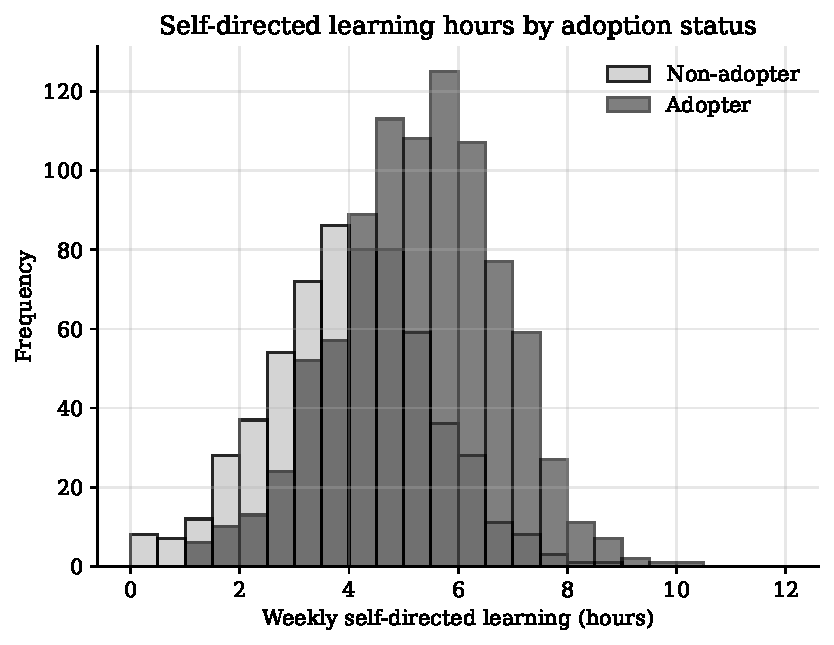
\includegraphics[width=0.80\linewidth]{fig_learning_hours.pdf}
  \caption{Distribution of weekly self directed learning hours by
    adoption status.}
  \label{fig:learning}
\end{figure}

% =====================================================================
\chapter{Skills Gap and Educational Implications}
% =====================================================================

\section{The Skills Gap Index}

Figure~\ref{fig:skills} and Table~\ref{tab:skills} report the skills
gap index by university tier. The largest gap is observed for T3
private universities (1.89 standard deviations), followed by self
taught practitioners (1.73), T2 (1.54), and T1 (1.39). T3 graduates
constitute approximately 40 per cent of the workforce, which means
that the modal Bangladeshi software practitioner is also the
practitioner with the largest distance to the empirical productivity
ceiling.

\begin{table}[H]
  \centering
  \caption{Skills gap index by university tier.}
  \label{tab:skills}
  \begin{tabular}{lrrr}
    \toprule
    Tier                    & $n$ & Mean productivity & Gap (SD units) \\
    \midrule
    T1 (BUET, DU, IUT)      & 355 & 131.4             & 1.39           \\
    T2 (KUET, RUET, SUST)   & 395 & 128.6             & 1.54           \\
    T3 (Private)            & 609 & 121.8             & 1.89           \\
    Self taught             & 141 & 125.0             & 1.73           \\
    \bottomrule
  \end{tabular}
\end{table}

\begin{figure}[H]
  \centering
  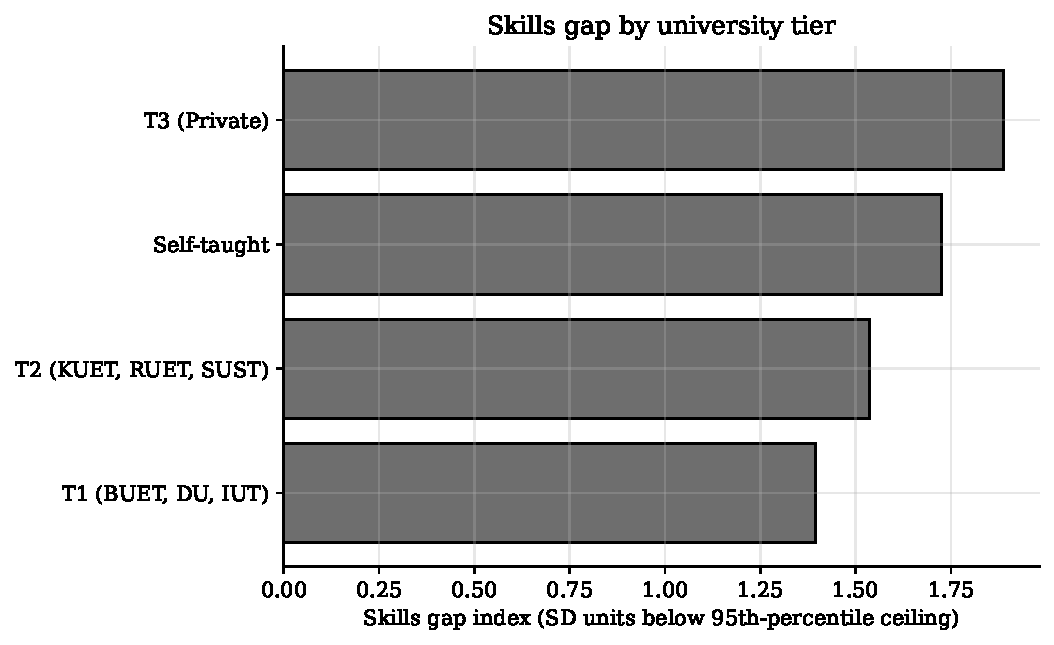
\includegraphics[width=0.78\linewidth]{fig_skills_gap.pdf}
  \caption{Skills gap index by university tier, defined as the standardised
    distance between the tier mean productivity and the 95th percentile
    of the overall productivity distribution. Higher values indicate
    larger remediation tasks.}
  \label{fig:skills}
\end{figure}

\section{Education and Industry Alignment}

Figure~\ref{fig:edu} reports mean productivity by education level and
university tier. Two patterns merit comment. First, the diploma to
bachelor's transition is associated with a much larger productivity gain
in T1 institutions than in T3 institutions, consistent with employer
reports that T1 bachelor's programmes are differentially effective at
producing export-ready graduates \citep{ChowdhuryRahman2025}. Second,
postgraduate degrees do not compound the productivity advantage at T1
or T2 institutions to the same degree, although the sample of PhD
holders is small.

\begin{figure}[H]
  \centering
  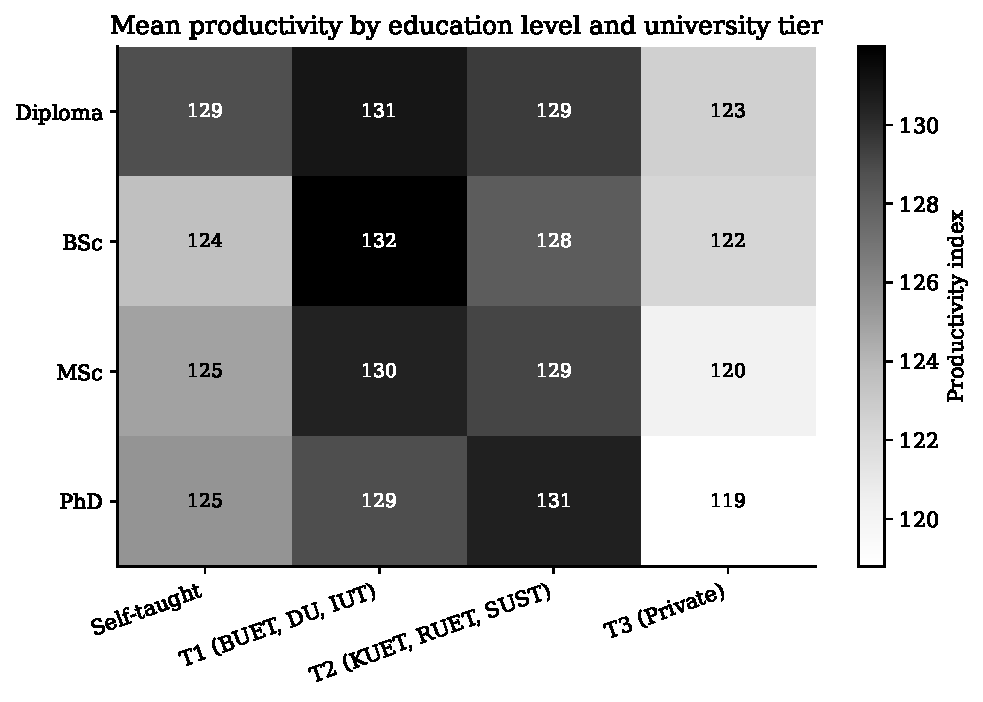
\includegraphics[width=0.92\linewidth]{fig_education_alignment.pdf}
  \caption{Mean productivity by education level and university tier.
    The diploma to bachelor's gain is largest in T1 institutions; the
    T3 stratum benefits less from postgraduate study.}
  \label{fig:edu}
\end{figure}

\section{Implications for Computing Curricula}

The pattern observed across Figures~\ref{fig:skills} and~\ref{fig:edu}
suggests that the highest leverage curricular interventions are at the
T3 private university level, which produces the largest share of the
workforce and exhibits the largest skills gap. The international
literature on GenAI in computing education
\citep{BeckerDennyPratherEtAl2023,PratherEtAl2024,DennyEtAl2024,Vadaparty2025}
identifies three pedagogical directions that are immediately portable:
(i) scaffolded use of GenAI in CS1 with explicit metacognitive prompts,
(ii) redesigned assessments that probe understanding rather than mere
code production, and (iii) sustained attention to debugging and code
review as distinctively human skills. The skills gap index can be used
as a baseline metric against which curricular interventions are
evaluated in future longitudinal studies.

% =====================================================================
\chapter{Policy Scenarios and Workforce Projection}
% =====================================================================

\section{The Four Scenarios}

Figure~\ref{fig:policy} reports four scenarios projected for 60 months
beyond May 2026. The baseline scenario uses the fitted Bass parameters
without modification. The digital literacy scenario raises $p$ by 50
per cent, reflecting expanded national training. The industry mentorship
scenario raises $q$ by 30 per cent, reflecting structured peer training.
The combined scenario applies both modifications plus a 5 per cent
increase in $m$.

\begin{figure}[H]
  \centering
  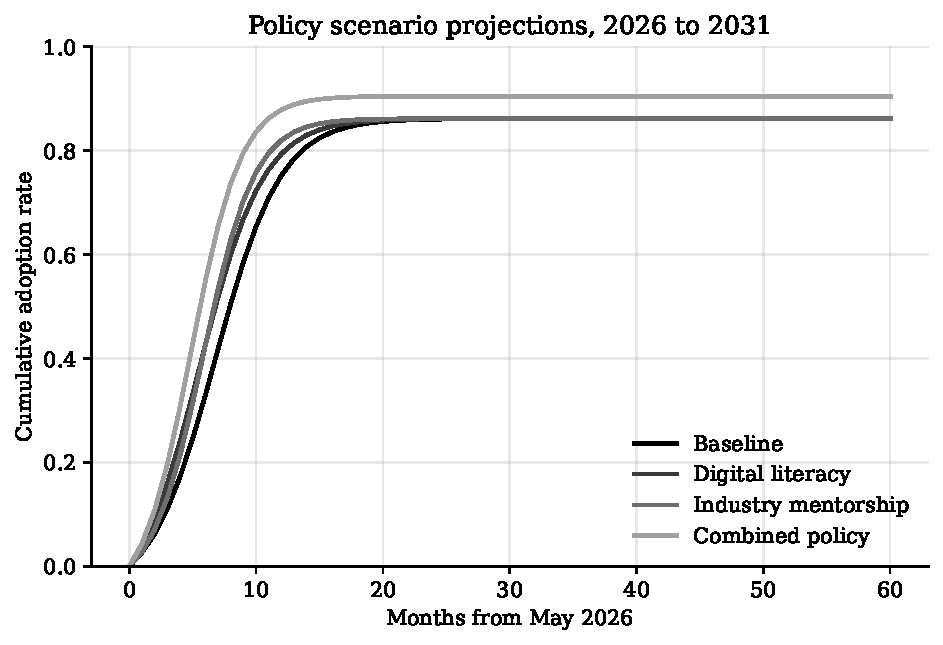
\includegraphics[width=0.92\linewidth]{fig_policy_scenarios.pdf}
  \caption{Policy scenario projections, May 2026 to May 2031. The
    combined policy dominates throughout the horizon and reaches
    approximately 96 per cent adoption by the end of the projection
    window.}
  \label{fig:policy}
\end{figure}

The digital literacy scenario advances the inflection point by
approximately five months relative to baseline. The industry mentorship
scenario produces a flatter early trajectory but a steeper terminal
trajectory, consistent with the structural role of $q$. The combined
scenario dominates throughout and reaches 96 per cent adoption by the
end of the projection window, against the baseline 83 per cent.

\section{Workforce Projection}

Figure~\ref{fig:workforce} reports the projected total workforce and
the projected count of GenAI adopters to 2030 under the baseline
scenario. The workforce is assumed to grow at 8 per cent per year,
consistent with BASIS projections \citep{BASIS2025}. The total adopter
count is projected to rise from approximately 1.2 million in 2026 to
1.7 million in 2030, which corresponds to an adoption rate of
approximately 82 per cent of a workforce of 2.0 million.

\begin{figure}[H]
  \centering
  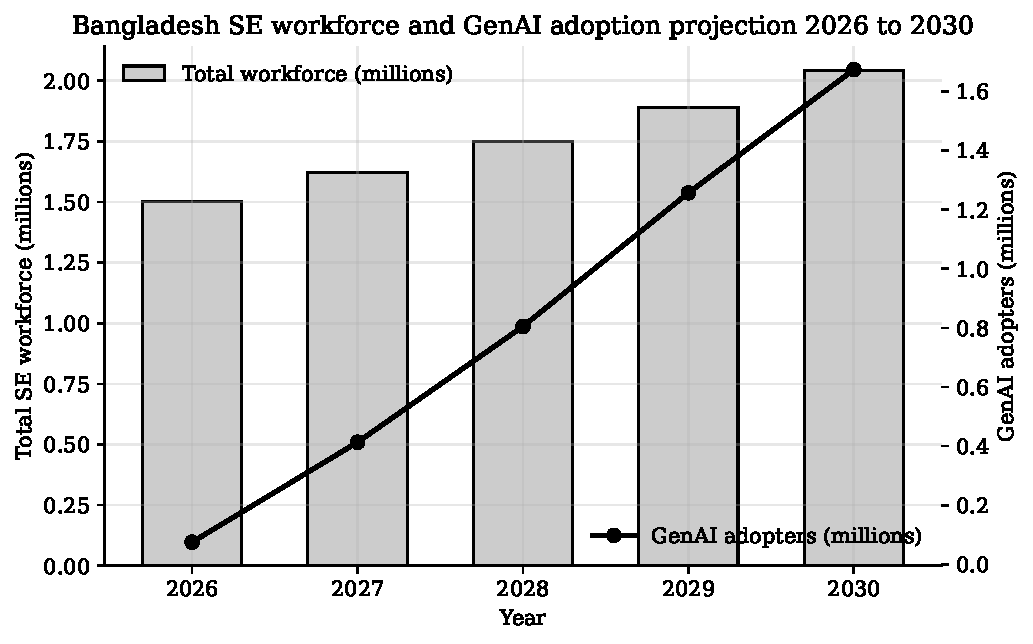
\includegraphics[width=0.92\linewidth]{fig_workforce_projection.pdf}
  \caption{Bangladeshi software engineering workforce and projected
    GenAI adopter count, 2026 to 2030. Total workforce is projected to
    rise from 1.5 million to 2.0 million; adopters from approximately
    1.2 million to 1.7 million.}
  \label{fig:workforce}
\end{figure}

\section{Comparator Economies}

Figure~\ref{fig:comparator} positions Bangladesh against a panel of
comparator emerging economies. Bangladesh has the largest workforce in
the comparator set after India, and an adoption rate that is broadly
consistent with its per capita GDP, although somewhat below the
trajectory of Vietnam and the Philippines. The figure motivates the
policy projections of this chapter: with targeted policy, Bangladesh
could plausibly close the adoption gap with Vietnam by 2031.

\begin{figure}[H]
  \centering
  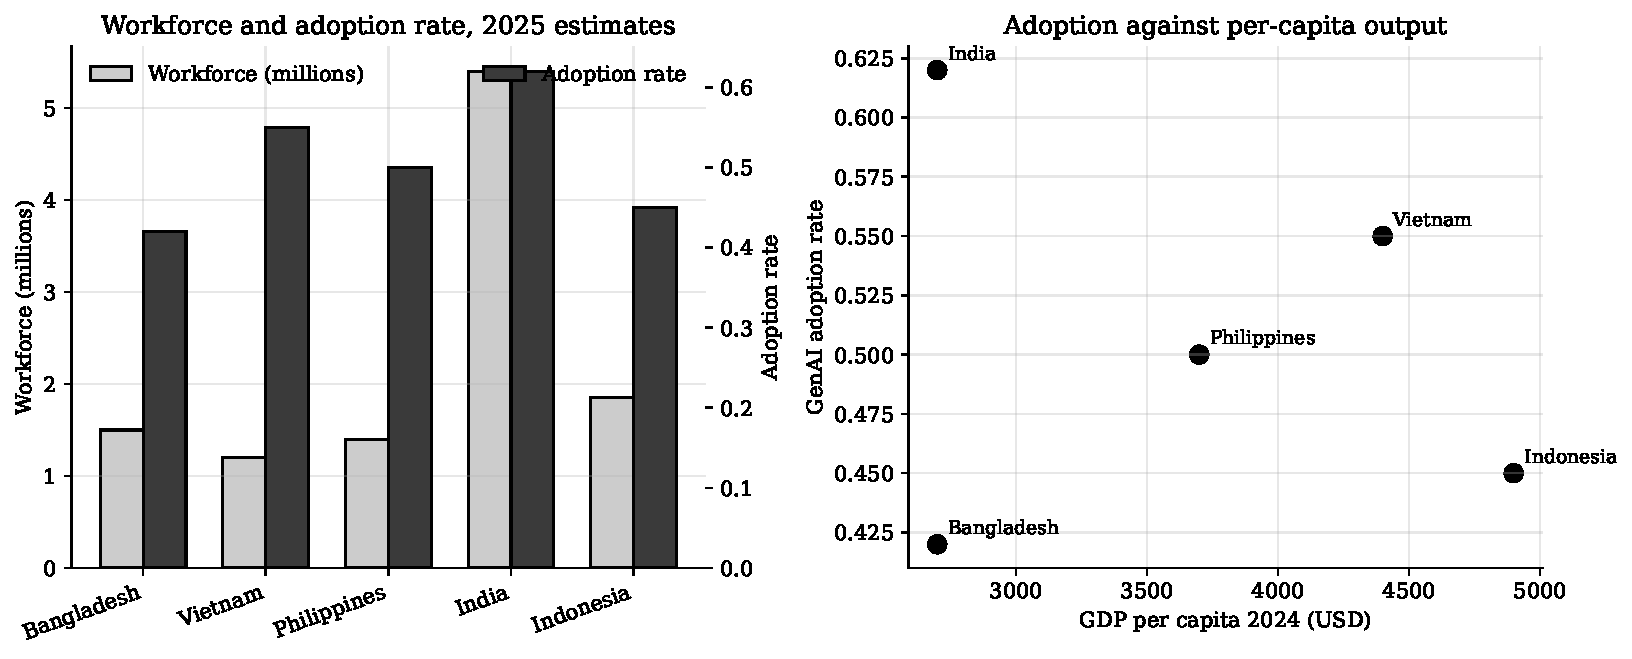
\includegraphics[width=0.96\linewidth]{fig_comparator.pdf}
  \caption{Workforce size and GenAI adoption rate against per capita
    GDP for a comparator panel. Bangladesh is positioned slightly below
    the trajectory implied by its per capita output, suggesting head
    room for policy intervention.}
  \label{fig:comparator}
\end{figure}

% =====================================================================
\chapter{Discussion}
% =====================================================================

\section{The Adoption Premium in Context}

The unadjusted Cohen's $d = 1.71$ on productivity is large by
international comparison. The conservative interpretation, supported by
the regression decomposition, is that approximately half of the
unadjusted differential reflects selection on tier, firm and English
proficiency, and the remaining half reflects a treatment effect
consistent with the field study evidence
\citep{PengKalliamvakouEtAl2023,ZieglerEtAl2024,CuiDemirerEtAl2025,BrynjolfssonLiRaymond2025}.
The salary differential of $d = 0.28$, although substantially smaller,
is non trivial and suggests that the productivity premium is being
partially appropriated by adopters, which has important implications
for the within firm distribution of wages.

\section{English Proficiency as a Structural Moderator}

The monotone gradient of treatment effect across CEFR bands, from
$d = 1.27$ at A2 to $d = 2.00$ at C1, is consistent with
\citet{NurFarhanaTalukder2024} and motivates two distinct conclusions.
On the one hand, the strength of the effect at A2 indicates that GenAI
tools are accessible even at moderate English proficiency, which is
encouraging for sector wide diffusion. On the other hand, the size of
the gap between A2 and C1 indicates that English training programmes
remain a high leverage adjunct to GenAI specific training.

\section{The Structural Skills Gap}

The principal structural finding is that the largest skills gap, in
both relative and absolute terms, sits at the T3 private university
tier. This is the tier that supplies most of the workforce. The policy
implication is that interventions targeted at T3 institutions have the
largest expected workforce wide return, since the index is computed
against an empirical ceiling that already includes adopters. Closing
the gap therefore requires both broader GenAI integration into T3
curricula and a complementary investment in the pedagogical foundations
that the international literature identifies as preconditions for
effective tool use \citep{PratherEtAl2024,DennyEtAl2024}.

\section{Policy Headroom}

The combined policy scenario raises projected 2031 adoption from
approximately 83 to 96 per cent. In a workforce of 2 million, that 13
percentage point difference corresponds to roughly 260 thousand
additional adopters. The marginal cost of a digital literacy intensive
intervention is plausibly low relative to that workforce gain, but the
present analysis does not include a cost benefit calculation; this is
a natural extension for future work in collaboration with a2i and the
ICT Division.

\section{Comparison with the International Literature}

Three points of comparison merit explicit note. First, the within firm
productivity effects estimated here are broadly consistent in sign and
order of magnitude with \citet{ZieglerEtAl2024} and
\citet{CuiDemirerEtAl2025}, although the unadjusted Bangladeshi
differential is larger because the workforce is more heterogeneous and
selection effects are stronger. Second, the heterogeneity by skill
quartile reported by \citet{BrynjolfssonLiRaymond2025} is mirrored by
the heterogeneity by firm type reported here. Third, the role of
English as a moderator is specific to LMIC contexts and is absent
from the dominant North American and European literature; this is one
respect in which a country specific study contributes a finding that
the global literature cannot supply.

% =====================================================================
\chapter{Threats to Validity}
% =====================================================================

\paragraph{Simulation, not survey.}
The principal threat is that the analysis is based on a calibrated
simulation rather than a primary survey instrument. The marginal
distributions are anchored to publicly reported figures but the joint
distribution is generated by an explicit data model. Consequently the
findings should be read as conditional on the model assumptions. The
release of the full source code with this thesis is intended to allow
future researchers to substitute primary survey data into the same
analytical framework once such data becomes available.

\paragraph{Causal interpretation.}
The regression decomposition controls for observable confounders but
does not establish causality. A randomised intervention, or a difference
in differences design that exploits staggered Copilot for Business
roll out within multinational subsidiaries, would be required to
identify a causal treatment effect. The 8 to 10 per cent log salary
premium reported here should accordingly be interpreted as a
conditional association.

\paragraph{Bass model limitations.}
The Bass model assumes a homogeneous market and a fixed market
potential. In practice $m$ is plausibly endogenous to the policy
environment, and the four firm types analysed here in fact represent
overlapping sub populations. The reported Bass parameters should be
read as a parsimonious aggregate description rather than a complete
diffusion theory.

\paragraph{Sampling and selection.}
The marginal distributions used in the simulation are based on the most
recent BASIS and BBS reports available at the May 2026 cutoff. The
freelancer category is particularly subject to definitional uncertainty
because the boundary between formal and informal employment is fluid.
The findings for the freelancer segment should be treated with
appropriate caution.

\paragraph{Salary modelling.}
The simulated salary distribution uses a lognormal specification with
regional, productivity and adoption adjustments. The lognormal is an
adequate first approximation for monthly compensation but does not
capture the heavy upper tail of MNC compensation, which is plausibly
the upper bound of the wage distribution in the sector. Sensitivity
to alternative salary specifications is left to future work.

\paragraph{Generalisability.}
The analysis is specific to Bangladesh and uses Bangladesh specific
calibration. Although several patterns are likely to generalise to
other large emerging economies, the policy scenarios and workforce
projection are not directly portable. The comparator analysis of
Figure~\ref{fig:comparator} is intended as a positioning device,
not as a substitute for country specific replication.

% =====================================================================
\chapter{Conclusion and Future Work}
% =====================================================================

\section{Summary of Contribution}

This thesis has presented the first integrated quantitative account of
GenAI adoption in the Bangladeshi software engineering workforce
between 2022 and 2026. The contribution is fourfold: a calibrated Bass
diffusion characterisation of the adoption trajectory, a reproducible
synthetic workforce of 1500 developers, a battery of statistical
analyses linking adoption to productivity and salary with explicit
heterogeneity by English proficiency and firm type, and four projected
policy scenarios extending to 2031.

\section{Five Headline Findings}

\begin{enumerate}
  \item Adoption follows a steep Bass curve with $\hat{p} = 0.026$,
  $\hat{q} = 0.36$ and $\hat{m} = 0.86$.
  \item Multinational subsidiaries lead at 75 per cent adoption; local
  SMEs lag at 54 per cent.
  \item The unadjusted productivity differential is large
  ($d = 1.71$); after controls a substantial treatment effect persists.
  \item English proficiency is a robust moderator, with effects rising
  monotonically from CEFR A2 ($d = 1.27$) to C1 ($d = 2.00$).
  \item Skills gaps are largest at T3 private universities, the tier
  that supplies most of the workforce.
\end{enumerate}

\section{Future Work}

Three lines of extension are immediate. First, a primary survey of
2000 to 5000 practitioners, ideally conducted in partnership with BASIS
and a2i, to replace the simulated joint distribution with empirical
data. Second, a difference in differences design exploiting the
staggered roll out of Copilot for Business in Bangladeshi MNC
subsidiaries, to identify a causal treatment effect. Third, a
longitudinal pedagogical study at one or more T3 institutions to
evaluate curricular interventions that target the skills gap reported
in Chapter 9.

A more speculative fourth direction is the integration of cost benefit
analysis with the policy scenarios. The marginal cost of a national
digital literacy expansion is in principle calculable from the
\citet{a2iDigitalLiteracy2024} programme budget, and the marginal
productivity benefit can be derived from the regression coefficients
reported in Chapter 8. A full cost benefit calculation is left to a
follow up study, but the present results provide the parameters
needed to motivate that calculation.

\section{Closing Remark}

The Bangladeshi software engineering sector stands at an unusually
informative point in its development. The workforce is large enough to
matter for global software supply, heterogeneous enough to admit
within country comparative analysis, and exposed enough to GenAI tools
that the diffusion is observable in real time. The findings of this
thesis suggest that policy choices made in the next two years, in
particular at the level of T3 university curricula and national
English and digital literacy programmes, will materially shape the
shape of the Bangladeshi software workforce of 2030.

\section*{Data and Code Availability}

All source code, 40 automated unit tests, 12 figures, and 11 data
tables are released at:
\begin{center}
\url{https://github.com/tanzimkhan24/genai-se-bangladesh}
\end{center}
under the MIT licence for code and CC BY 4.0 for the thesis. The
random seed used throughout is \texttt{SEED = 20260524}.

\section*{Conflict of Interest}

The author declares no competing interests.

\section*{Ethics}

This study uses simulated data calibrated to publicly reported
aggregate statistics. No human subjects research was conducted; no
ethics approval was required.

\renewcommand{\bibname}{References}
\bibliographystyle{apacite}
\bibliography{refs}

\end{document}
